\documentclass{uebblatt}
\usepackage{wrapfig}

\newcommand{\cont}{\mathrm{cont}}
\newcommand{\http}{http:/\kern-.2em/\kern-0.03em}

\begin{document}

\maketitle{13}{}

\begin{aufgabe}{m+2}{Ein Erstsemestertraum wird wahr}
Sei ein Ring~$A$ mit der adischen Topologie bezüglich einem
Ideal~$\aaa$ versehen.
Sei~$(x_n)_n$ eine Folge in~$A$. Sei~$s_n = \sum_{k=0}^n x_k$.
Zeige: Genau dann ist~$(s_n)_n$ eine Cauchy-Folge,
wenn~$(x_n)_n$ eine Nullfolge ist.
\end{aufgabe}

%\begin{aufgabe}{}{Zu schön um wahr zu sein?}
%Sei~$x$ ein Element eines topologischen Rings. Gelte~$x^n \xrightarrow{n \to
%\infty} 0$. Ist~$x$ nilpotent?
%\end{aufgabe}

\begin{aufgabe}{3}{Abgeschlossenheit maximaler Ideale}
Sei~$\aaa$ ein Ideal in einem Ring~$A$. Zeige, dass ein maximales Ideal~$\mmm$
von~$A$ genau dann abgeschlossen bezüglich der~$\aaa$-adischen Topologie
auf~$A$ ist, wenn~$\aaa \subseteq \mmm$.
\end{aufgabe}

\begin{aufgabe}{m}{Vervollständigung an maximalen Idealen}
Sei~$\mmm$ ein maximales Ideal in einem Ring~$A$. Zeige, dass die
Vervollständigung von~$A$ bezüglich der~$\mmm$-adischen Topologie ein lokaler
Ring ist.
\end{aufgabe}

\begin{aufgabe}{2+m}{Analytische Umgebungen}
Sei~$K$ ein Körper mit~$2 \neq 0$.
\begin{enumerate}
\item Zeige: $\psxy{K}/(y^2-x^2) \cong \psxy{K}/(y^2-x^2-x^3)$.
\item Zeige: $K[X,Y]/(y^2-x^2) \not\cong K[X,Y]/(y^2-x^2-x^3)$.
\end{enumerate}
\end{aufgabe}

\setlength{\wrapoverhang}{1.3cm}
\setlength{\columnsep}{0.8cm}
\begin{wrapfigure}{r}{0.35\textwidth}
  \vspace{-6em}
  \scriptsize
  \[ \xymatrix{
    & \vdots \ar[d]_p & \vdots \ar[d]^\id & \vdots \ar[d] \\
    0 \ar[r] & \ZZ \ar[r]^{p^3}\ar[d]_p & \ZZ \ar[r]\ar[d]^\id & \ZZ/(p^3) \ar[r]\ar[d] & 0 \\
    0 \ar[r] & \ZZ \ar[r]^{p^2}\ar[d]_p & \ZZ \ar[r]\ar[d]^\id & \ZZ/(p^2) \ar[r]\ar[d] & 0 \\
    0 \ar[r] & \ZZ \ar[r]^p & \ZZ \ar[r] & \ZZ/(p) \ar[r] & 0
  } \]
\end{wrapfigure}

\begin{aufgabe}{2+2}{Nichtexaktheit der inversen Limesbildung}
Das Diagramm zeigt in seinen drei Spalten drei inverse
Systeme~$A_\bullet$,~$B_\bullet$ und~$C_\bullet$ und horizontal die Komponenten
einer kurzen exakten Sequenz~$0 \to A_\bullet \to B_\bullet \to C_\bullet \to 0$.
\begin{enumerate}
\item Bestimme die inversen Limiten der drei Systeme.
\item Ist~$\lim^1 A_\bullet = 0$? Beschreibe~$\lim^1 A_\bullet$ so gut wie
möglich!
\end{enumerate}
\end{aufgabe}

\begin{aufgabe}{0}{Die 10-adischen Zahlen}
Finde ein Element~$x \in \ZZ_{10}$, das weder Null noch Eins ist, aber trotzdem
die Identität~$x^2 = x$ erfüllt. Kann ein Grundschulkind die ersten paar
Ziffern von~$x$ bestimmen?
\end{aufgabe}

\centering
\rotatebox{90}{\tiny\sffamily \http brownsharpie.courtneygibbons.org/?p=46}
\href{http://brownsharpie.courtneygibbons.org/?p=46}{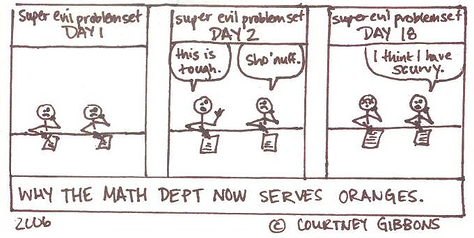
\includegraphics[scale=1.2]{images/super-evil-problem-set}}

\end{document}

Aufgabe 10.3 im Skript?

\hat A_a = A[[x_1,...,x_n]]/(x_i-a_i) für a = (a_1,...,a_n) und A noethersch?
http://www.math.uchicago.edu/~may/MISC/Topologies.pdf

In Z_p gibt es keine Wurzel aus p. Lokal-zu-global-Prinzip.

Schön wäre noch: eine Aufgabe zu Artin--Reese und Co.
